\chapter{Design}
\textbf{Versionshistorik}
\begin{longtabu} to \linewidth{@{}l l l X[j]@{}}
    Version &    Dato &    Ansvarlig &    Beskrivelse\\[-1ex]
    \midrule
    1.0		&	 &		&	\\[-1ex]
\label{version_Systemark}
\end{longtabu}

\section{Systemarkitektur} 
Igennem BBD og IBD vil det overordnede blodtryksmålersystem beskrives i forhold til hvilke blokke systemet består af, og hvordan de interagerer med hinanden. 

\subsection{BBD-diagram}
På figur 2.1 ses BDD-diagrammet for systemet. BBD viser de forskellige blokke for systemet og hvilke porte de består af. I tabel 2.2 ses en beskrivelse af blokkene. 

\begin{figure}[H]
	\centering
	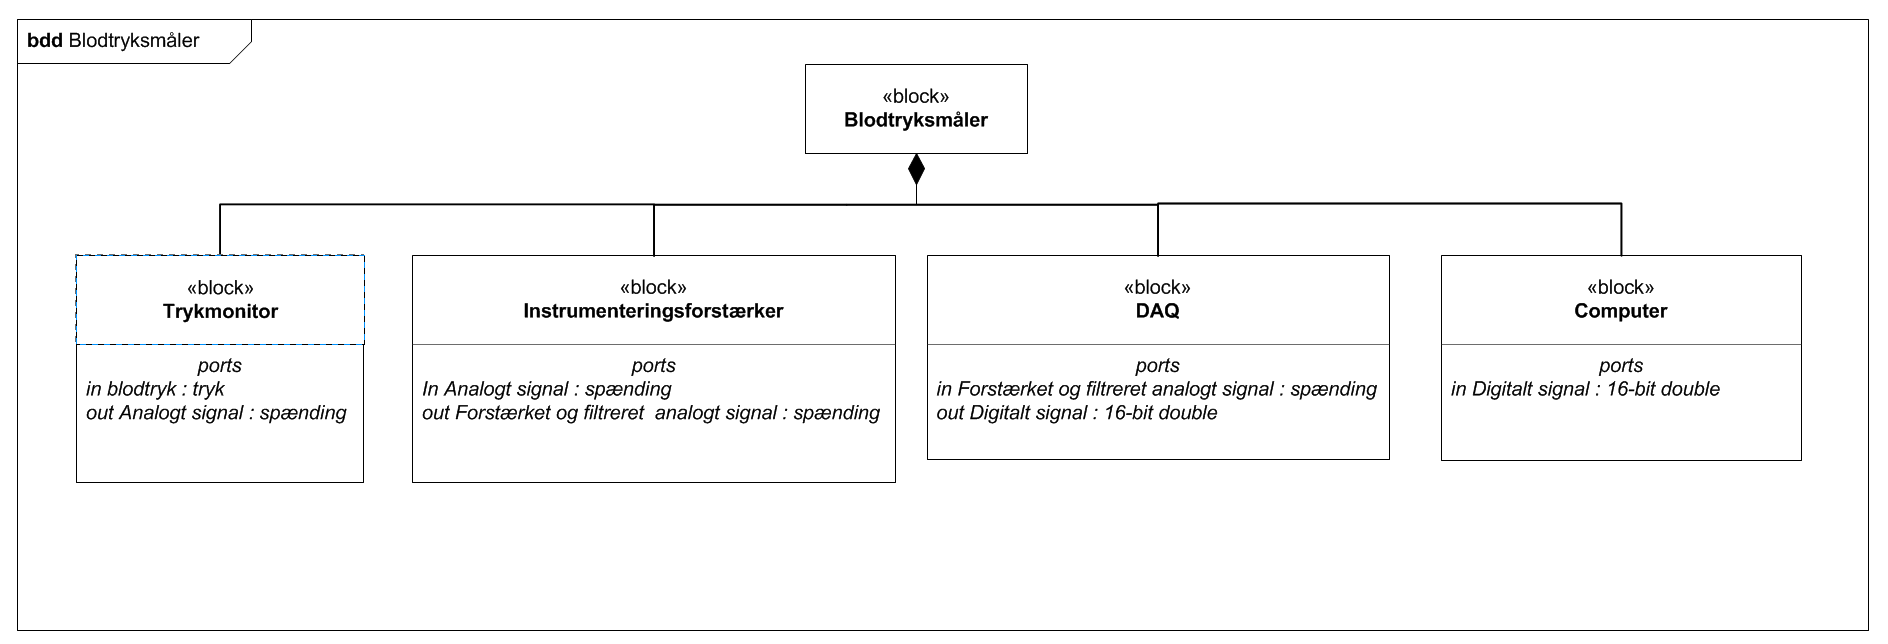
\includegraphics[width=1\textwidth]{Figurer/Snip20151102_8}
	\caption{BBD-diagram}
	\label{fig:BBD-diagram}
\end{figure}

\begin{longtabu} to \linewidth{@{}l X[j]@{}}
	\textbf{Blok} &	\textbf{Beskrivelse} \\[-1ex]
	\midrule
	Blodtryksmåler & Det overordnede system, som indeholder Trykmonitor, Instrumenteringsforstærker, DAQ og Computer\\[-1ex]
	Trykmonitor & Registrerer en fysisk størrelse i form af en trykændring. I dette system anvendes en transducer. Transduceren har til opgave at transformere den fysiske størrelse til en elektrisk spænding, som viderebehandles gennem de resterne hardware blokke  \\[-1ex]
	Instrumenteringsforstærker & Består af to dele. En forstærker-del og en filterings-del. Det analoge signal fra Trykmonitoren bliver via denne blok forstærket og filteret\\[-1ex]
	DAQ & Konverterer det analoge signal fra Trykmonitoren til et digitalt signal\\[-1ex]
	Computer & Indeholder software til systemet, som er kodet i Visual Studio C\#. Softwaren kan blandt andet vise det digitale signal grafisk. Softwaren kan ligeledes kalibrere, nulpunktsjustere og gemme målinger samt aktivere og deaktiver filter\\[-1ex]
	\caption{Beskrivelse af blokkene for systemet}
	\end{longtabu}
	
\subsection{IBD-diagram}
På figur 2.2 ses IBD-diagrammet for systemet. IBD viser, hvordan de forskellige blokke intergerer med hinanden. IBD fortæller signalets behandling gennem systemet - altså hvordan signalet transformeres fra et målt fysisk tryk til et digitalt signal, som softwaren kan videre behandle og vise grafisk. 

\begin{figure}[H]
	\centering
	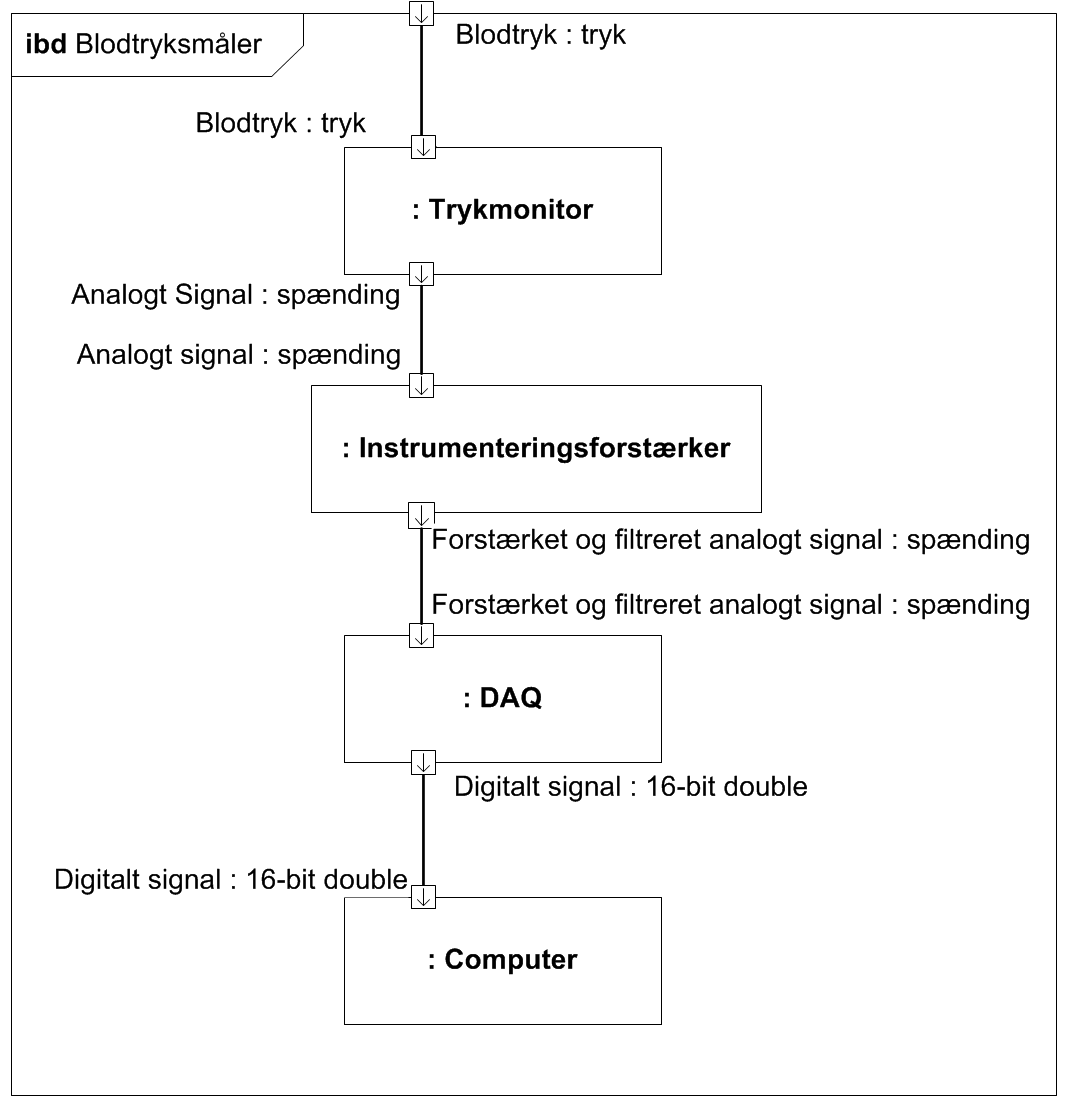
\includegraphics[width=0.8\textwidth]{Figurer/Snip20151102_7}
	\caption{IBD-diagram}
	\label{fig:IBD-diagram}
\end{figure}

\section{Grænseflader}
Kommunikationsprotokol for hardware blokkene ses i tabel 2.3. Det er en beskrivelse og specifikation af hvilken indgang- og udgangssignal de forskellige blokke har.   

\begin{longtabu} to \linewidth{@{}l l l l X[j]@{}}
	\textbf{Grænseflade} & \textbf{Signal} & \textbf{Type} & \textbf{Format} & \textbf{Værdi} \\[-1ex]
	\midrule
	Trykmoniter & Blodtryk & in & Tryk & 0 - 300 mmHg \\[-1ex]
				& Analogt & out & Spænding & +/- 13,5mV \\[-1ex]
	Forstærker  & Analogt & in & Spænding & +/- 13,5mV \\[-1ex]
				& Forstærket analogt & out & Spænding & +/- 5V \\[-1ex]
	Filter 		& Forstærket analogt & in & Spænding & +/- 5V \\				[-1ex]
				& Filteret analogt & out & Spænding & +/- 5V \\[-1ex]
	DAQ			& Filteret analogt & in & Spænding & +/- 5V \\				[-1ex]	
				& Digitalt & out & 16-bit double & +/- 5 \\[-1ex]
	Computer	& Digitalt & in & 16-bit double & +/- 5 \\[-1ex]
	\caption{Kommunikationsprotokol}	
\end{longtabu}


\section{Hardware arkitektur}


\section{Software arkitektur}

\subsection{Domænemodel}

\subsection{Applikationsmodel}

\subsubsection{Sekvensdiagram}
Sekvensdiagrammerne beskriver step-by-step, via metoder, forløbet i de forskellige Use Cases. Der er lavet et sekvensdiagram for hver Use Case, for at gøre systemet mere overskueligt. Et sekvensdiagram består af boundary-klasserne og domain-klasserne fra domænemodellen, samt en controller-klasse, med navn efter den specifikke Use Case.

\begin{figure}[H]
	\centering
	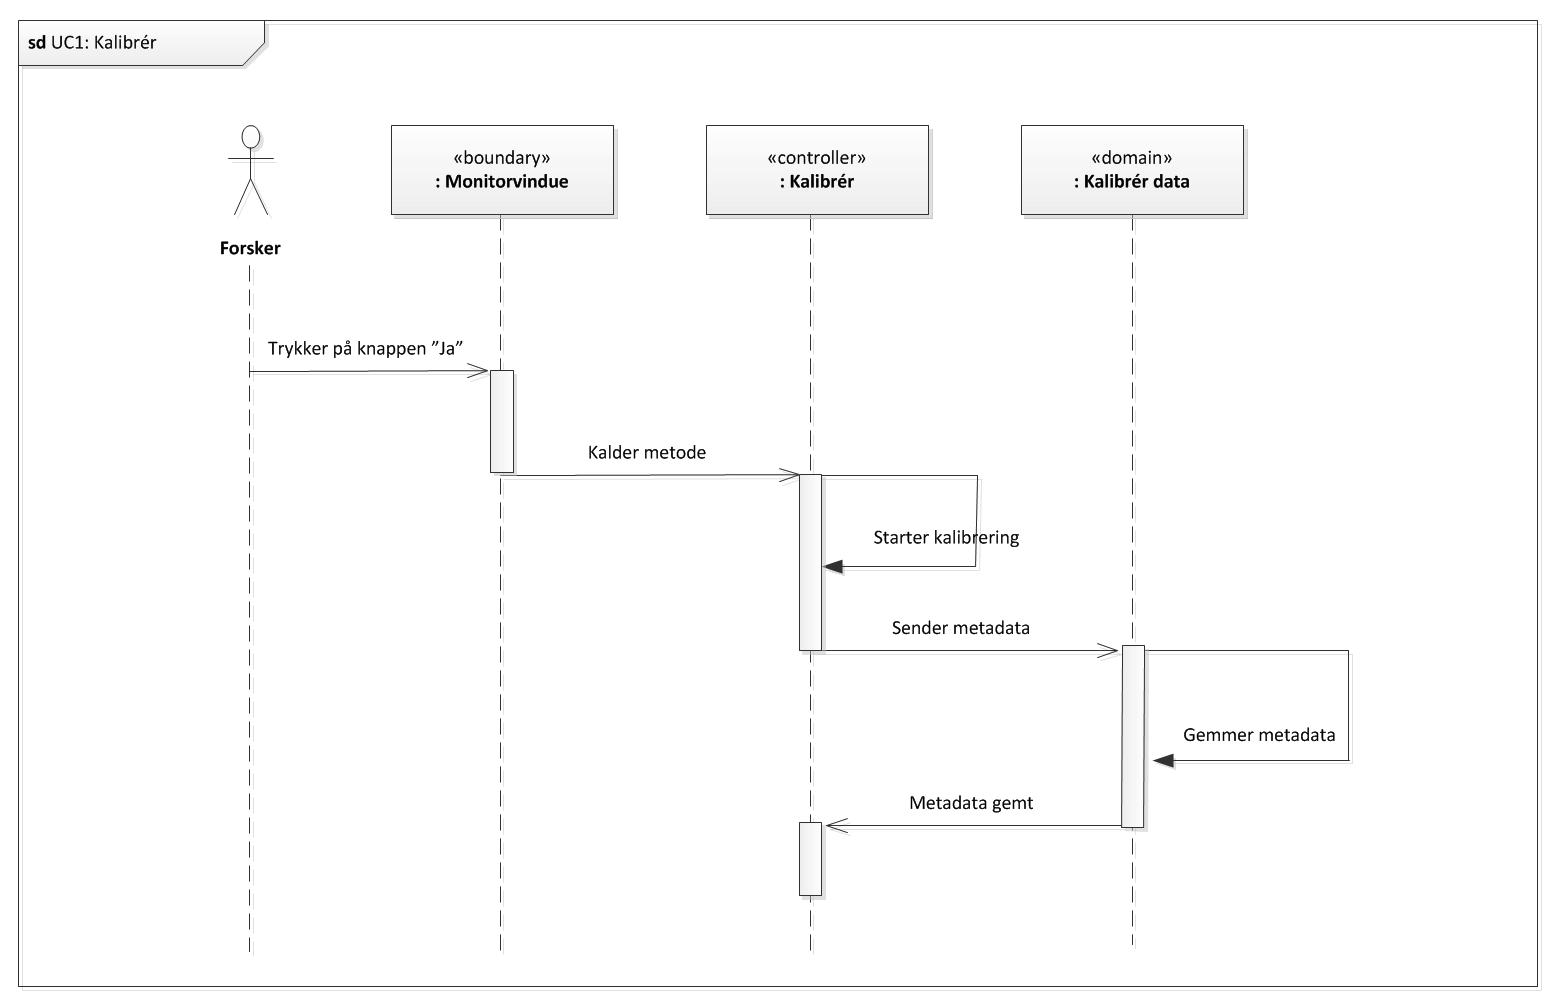
\includegraphics[width=1\textwidth]{Figurer/Snip20151102_9}
	\caption{Sekvensdiagram for UC1}
\end{figure}

\begin{figure}[H]
	\centering
	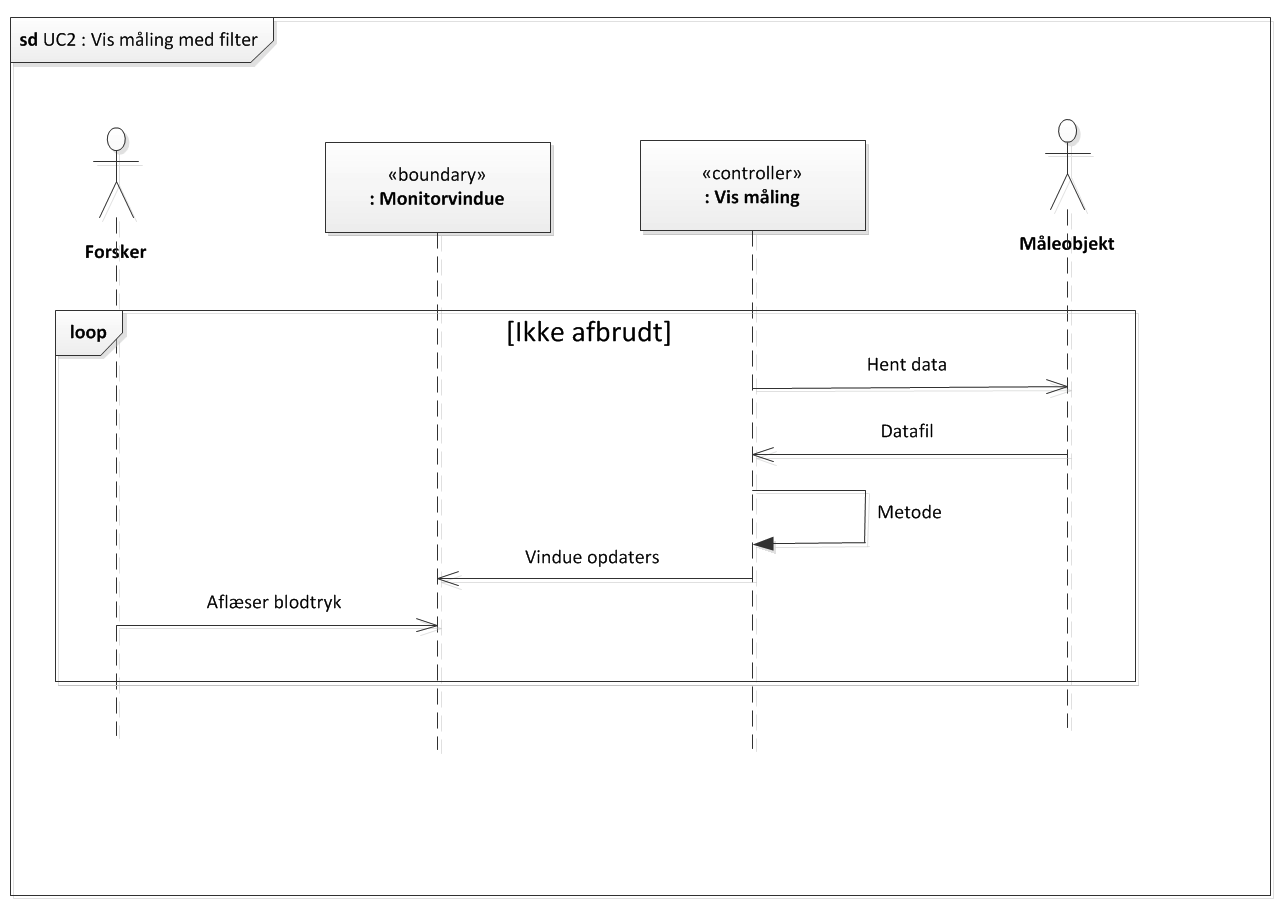
\includegraphics[width=1\textwidth]{Figurer/Snip20151102_10}
	\caption{Sekvensdiagram for UC2}
\end{figure}

\begin{figure}[H]
	\centering
	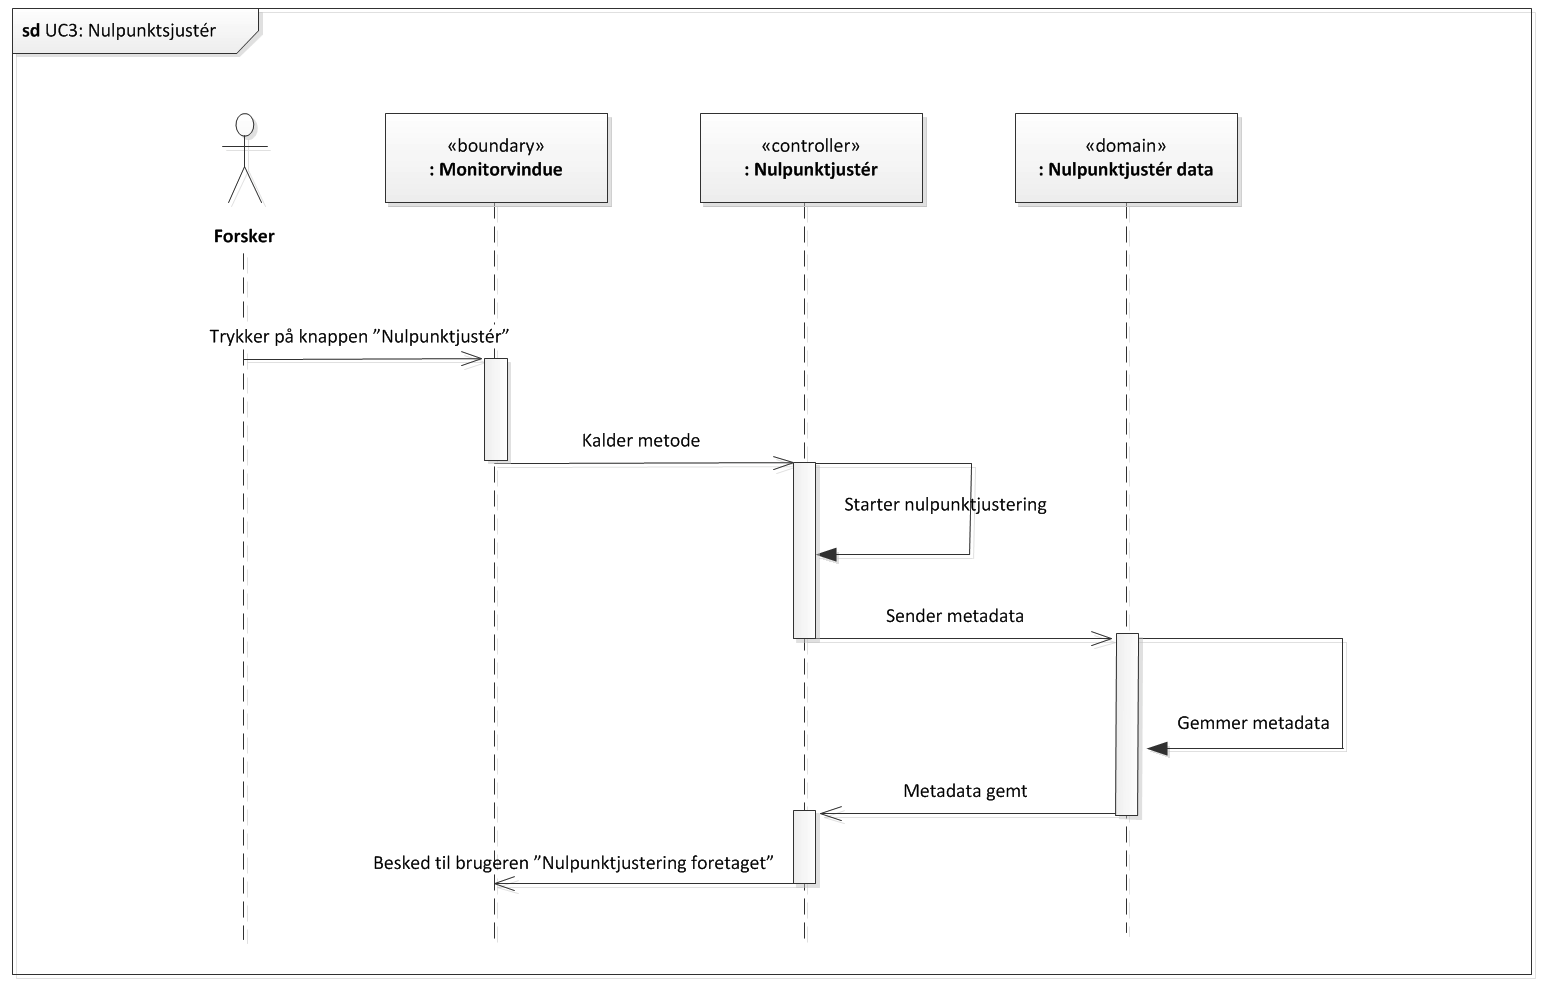
\includegraphics[width=1\textwidth]{Figurer/Snip20151102_11}
	\caption{Sekvensdiagram for UC3}
\end{figure}

\begin{figure}[H]
	\centering
	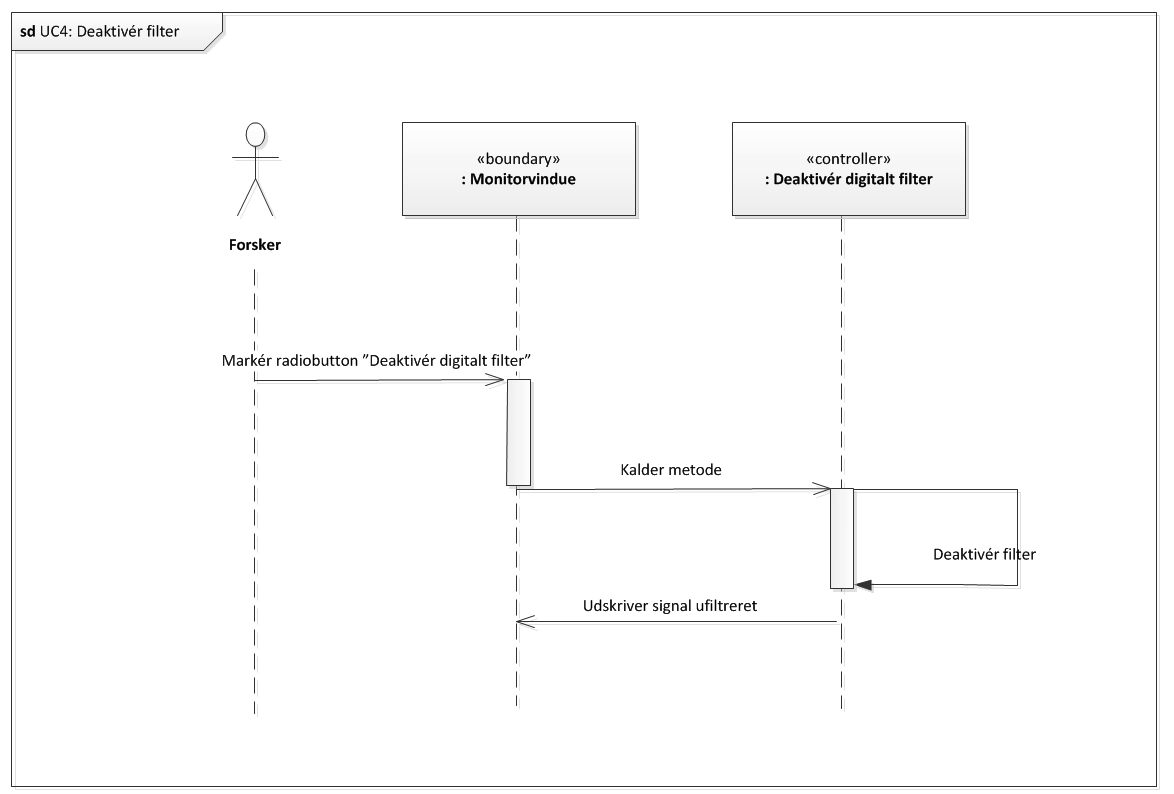
\includegraphics[width=1\textwidth]{Figurer/Snip20151102_12}
	\caption{Sekvensdiagram for UC4}
\end{figure}

\begin{figure}[H]
	\centering
	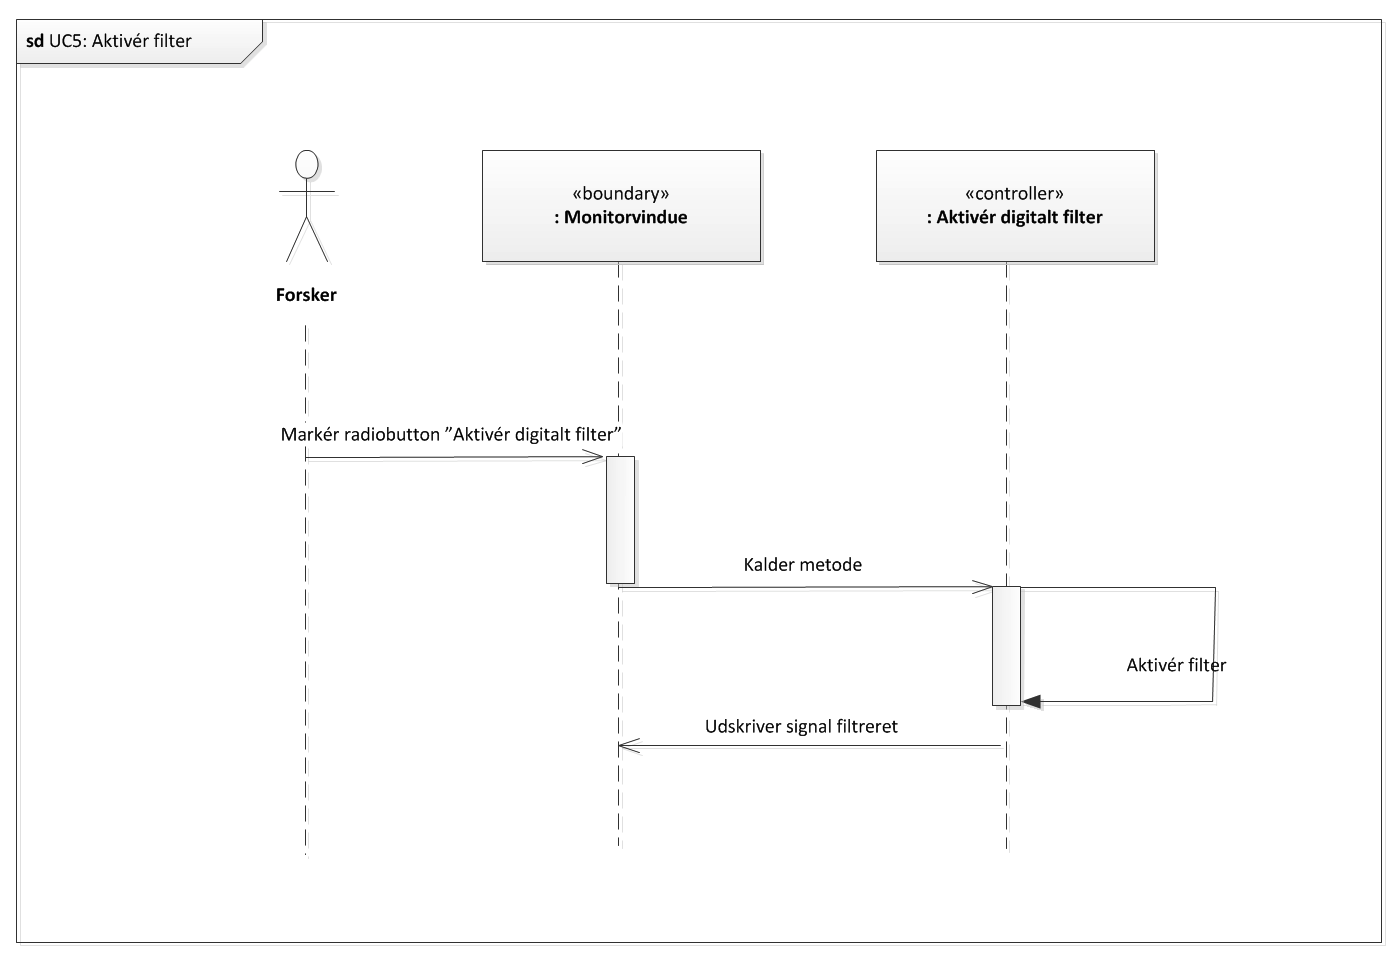
\includegraphics[width=1\textwidth]{Figurer/Snip20151102_13}
	\caption{Sekvensdiagram for UC5}
\end{figure}

\begin{figure}[H]
	\centering
	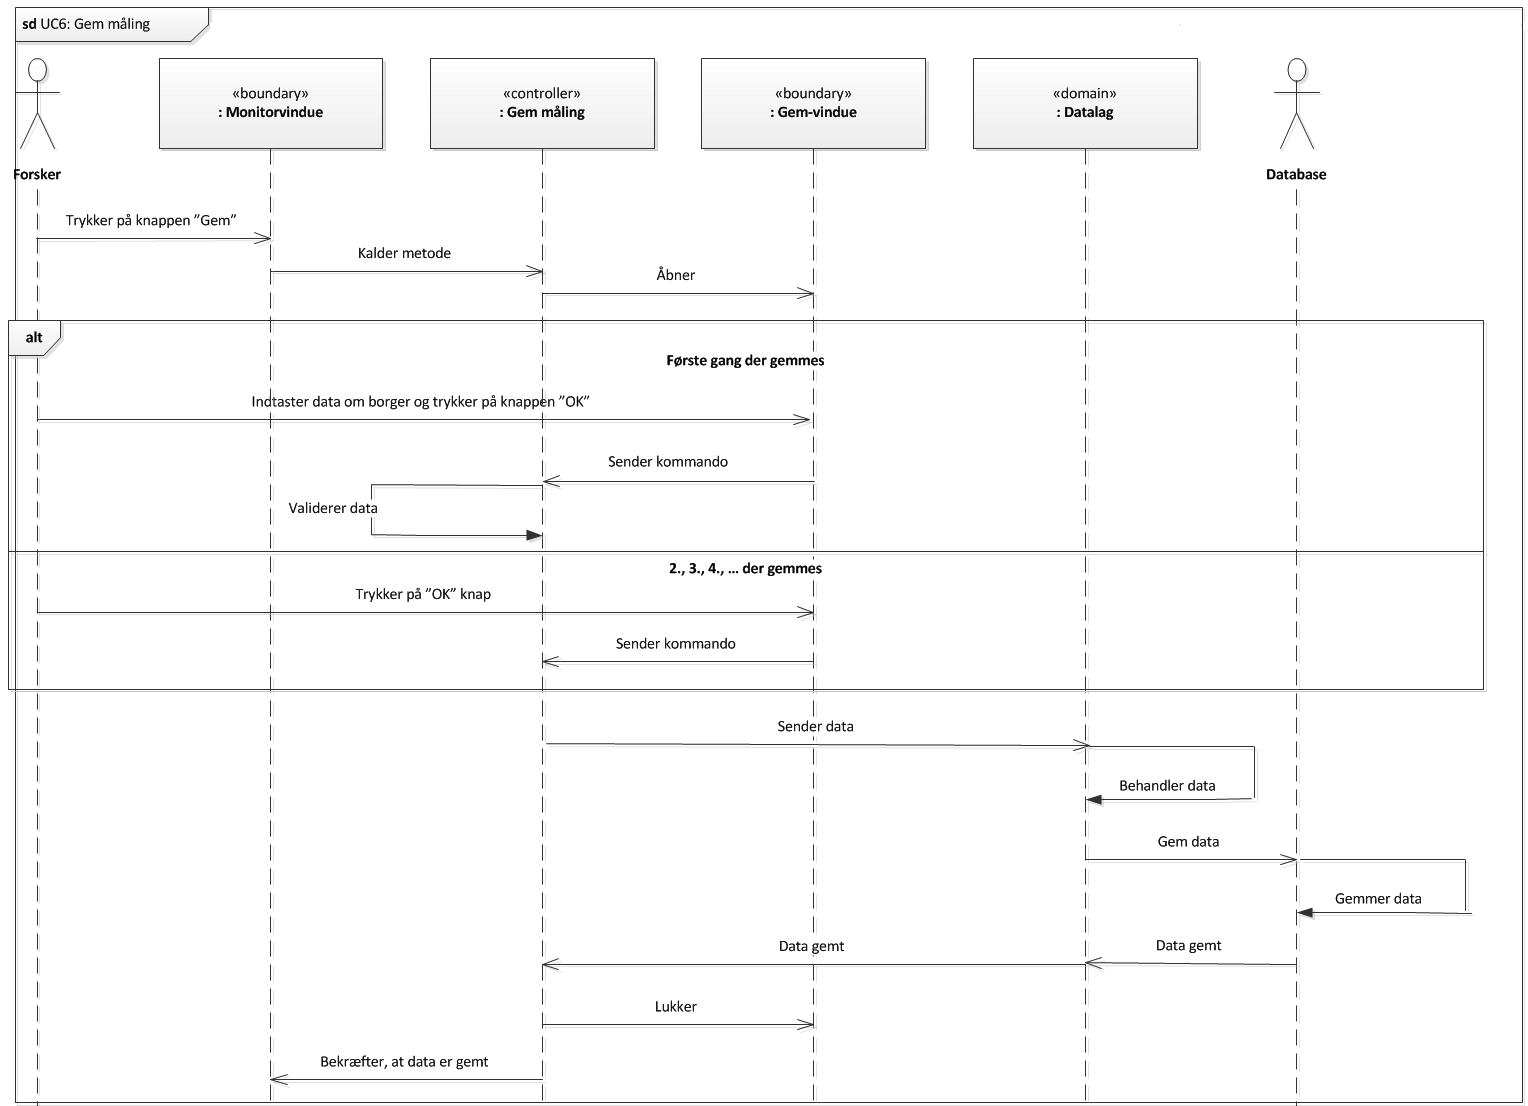
\includegraphics[width=1\textwidth]{Figurer/Snip20151102_14}
	\caption{Sekvensdiagram for UC6}
\end{figure}

\subsubsection{Opdateret klassediagram}
De opdateret klassediagrammer indeholder metoderne fra de dertilhørende  sekvensdiagrammer - dette giver et overblik over, hvilke metoder de forskellige klasser består af.

\begin{figure}[H]
	\centering
	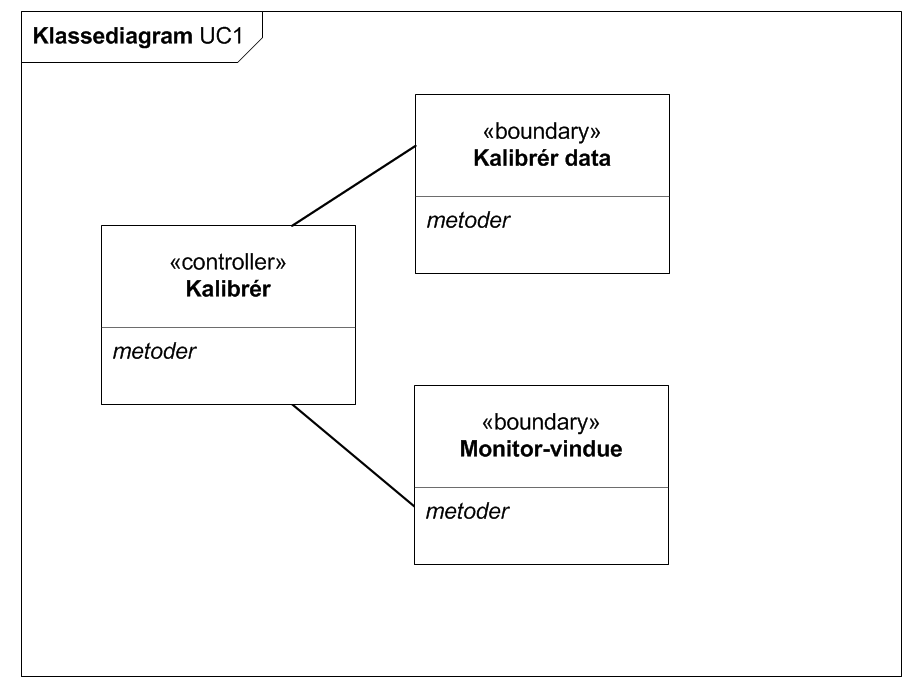
\includegraphics[width=1\textwidth]{Figurer/Snip20151102_15}
	\caption{Klassediagram for UC1}
\end{figure}

\begin{figure}[H]
	\centering
	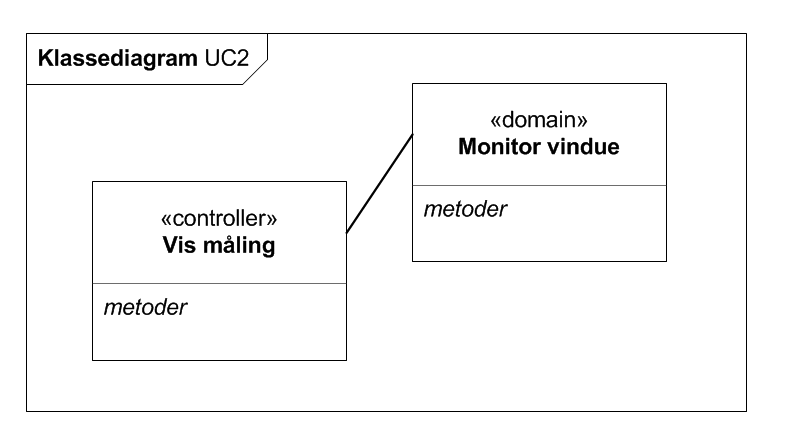
\includegraphics[width=1\textwidth]{Figurer/Snip20151102_16}
	\caption{Klassediagram for UC2}
\end{figure}

\begin{figure}[H]
	\centering
	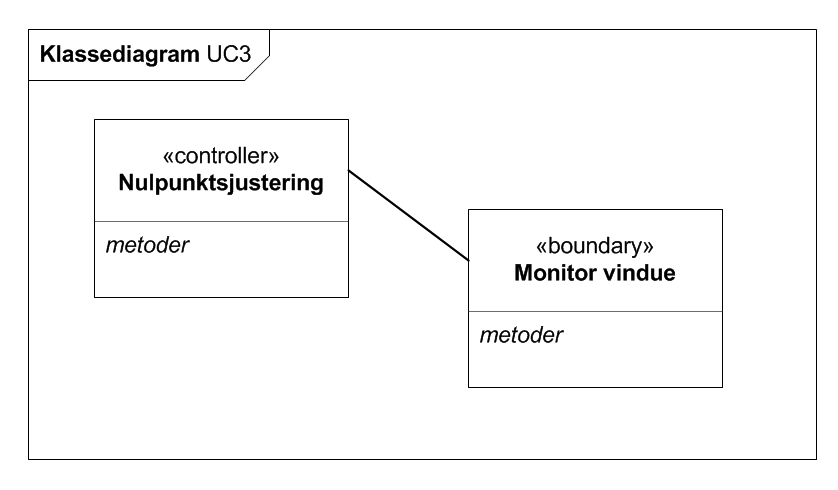
\includegraphics[width=1\textwidth]{Figurer/Snip20151102_17}
	\caption{Klassediagram for UC3}
\end{figure}

\begin{figure}[H]
	\centering
	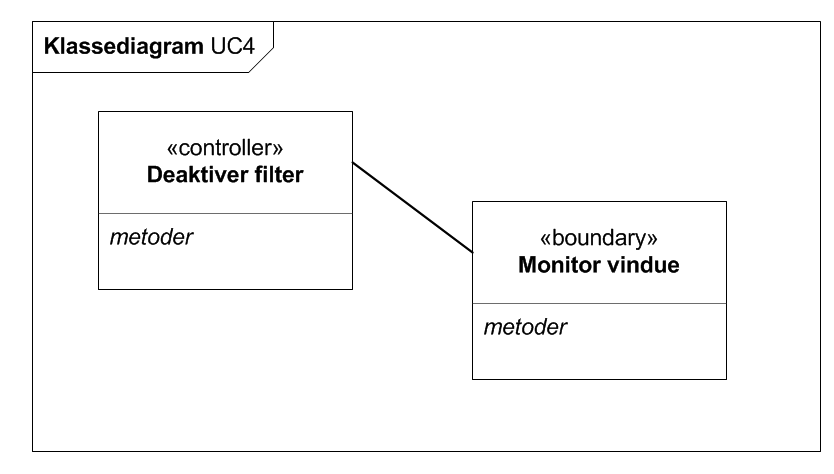
\includegraphics[width=1\textwidth]{Figurer/Snip20151102_18}
	\caption{Klassediagram for UC4}
\end{figure}

\begin{figure}[H]
	\centering
	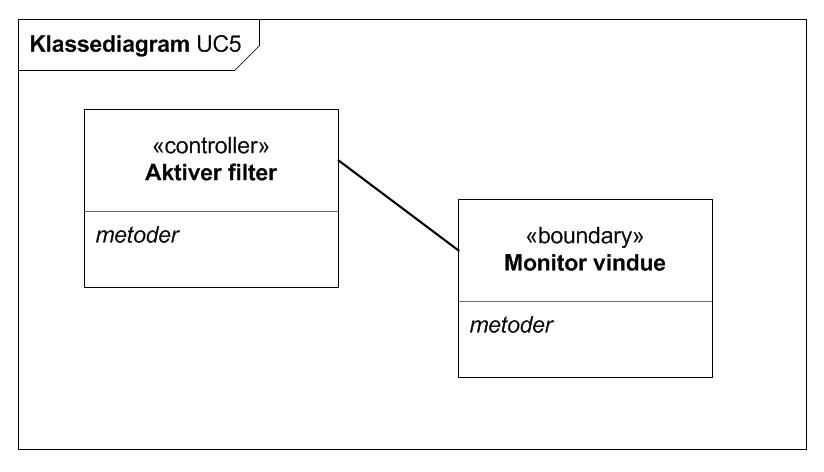
\includegraphics[width=1\textwidth]{Figurer/Snip20151102_19}
	\caption{Klassediagram for UC5}
\end{figure}

\begin{figure}[H]
	\centering
	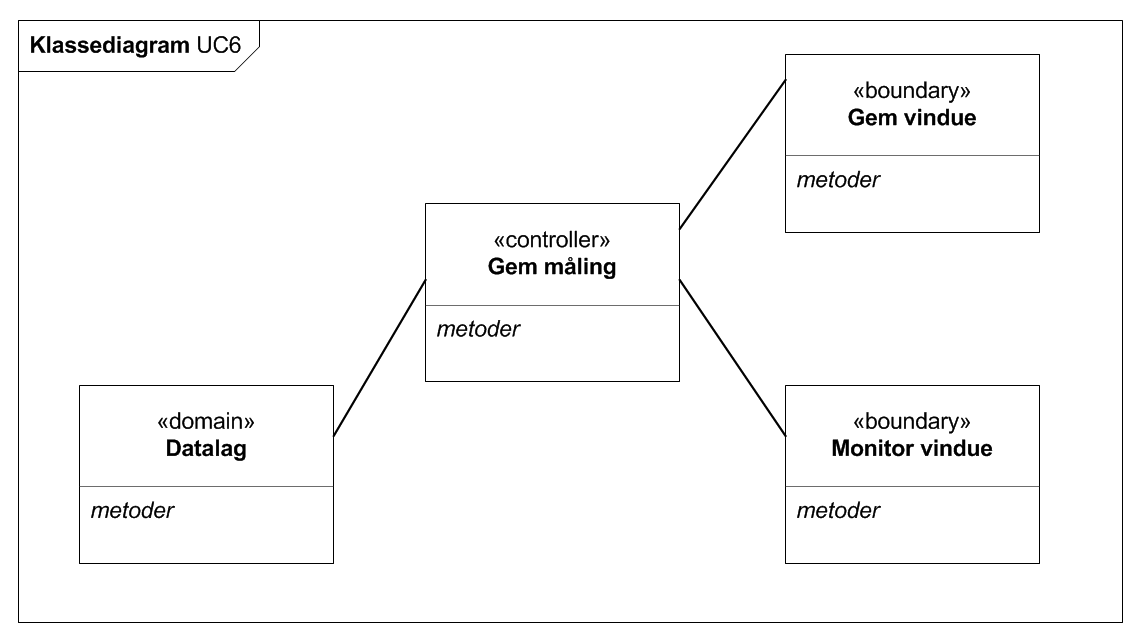
\includegraphics[width=1\textwidth]{Figurer/Snip20151102_20}
	\caption{Klassediagram for UC6}
\end{figure}












